\documentclass[a4paper, 12pt]{article}
\usepackage[brazil]{babel}
\usepackage[utf8]{inputenc}
\usepackage{indentfirst}
\usepackage{graphicx}
\usepackage[font=footnotesize,labelfont=bf]{caption} %muda o tamanho das caption e deixa em negrito
\usepackage{cite}
\usepackage{color}   %May be necessary if you want to color links
\usepackage{hyperref}
\hypersetup{
    colorlinks=true,
    citecolor=blue,
    filecolor=blue,
    linkcolor=blue,
    urlcolor=blue
}
\usepackage{listings}
\renewcommand{\lstlistingname}{Algoritmo}
% \definecolor{codegreen}{rgb}{0,0.6,0}
\definecolor{codegray}{rgb}{0.5,0.5,0.5}
% \definecolor{codepurple}{rgb}{0.58,0,0.82}
\definecolor{backcolour}{rgb}{0.95,0.95,0.92}
\lstdefinestyle{mystyle}{
    backgroundcolor=\color{backcolour},   
    % commentstyle=\color{codegreen},
    % keywordstyle=\color{magenta},
    numberstyle=\tiny\color{codegray},
    % stringstyle=\color{codepurple},
    basicstyle=\footnotesize,
    breakatwhitespace=false,         
    breaklines=true,                 
    captionpos=b,                    
    keepspaces=true,                 
    numbers=left,                    
    numbersep=5pt,                  
    showspaces=false,                
    showstringspaces=false,
    showtabs=false,                  
    tabsize=2
}
\lstset{style=mystyle}

\begin{document}
\begin{titlepage}
    \begin{center}
		\LARGE{Universidade Federal de Mato Grosso do Sul}\\
		\vspace{5pt}
        \large{Campus Ponta Porã}\\ 
        \large{{\textbf{Análise de Algoritmos I}}}\\ 
        \vspace{15pt}
        \vspace{95pt}
        \textbf{\large{Trabalho Prático II}}\\
        \vspace{15pt}
        \textbf{\LARGE{Problema da Mochila Booleana}}\\
        %\title{{\large{Título}}}
        \vspace{3,5cm}
    \end{center}
    
    \begin{flushleft}
        \begin{tabbing}
            Aluno: Daniel de Leon Bailo da Silva\\            
            Professor: Eduardo Theodoro Bogue\\
            %Professor co-orientador: \\
    \end{tabbing}
 \end{flushleft}
    \vspace{1cm}
    
    \begin{center}
        \vspace{\fill}
            Maio\\
         2019
            \end{center}
\end{titlepage}

\clearpage
\tableofcontents
\thispagestyle{empty}
\clearpage

% ref
% https://en.wikibooks.org/wiki/LaTeX/Labels_and_Cross-referencing
% tabela
% https://www.tablesgenerator.com/#

\pagenumbering{arabic}
\section*{Resumo}
\addcontentsline{toc}{section}{Resumo}
\label{sec:resumo}
Este trabalho consiste em mostrar os resultados obtidos a partir da execução
do algoritmo da {\it Mochilha Boolena} ou {\it Knapsack 0/1}, em suas versões dinâmicas.
Feito isso, dada as instâncias para aplicar os algoritmos, foi comparado o tempo de execução para cada instância 
nas suas versões dinâmicas, {\it Top-Down} e  {\it Bottom-Up}.\\

{\bf Considerar o seguinte ambiente para a obtenção dos resultados:}
\begin{itemize}
    \item Processador: Intel Core™ i5-8250U
    \begin{itemize}
        \item Número de núcleos 4
        \item Número de threads 8
        \item Frequência baseada em processador 1.60 GHz
        \item Frequência turbo max 3.40 GHz
    \end{itemize}
    \item Memória: 8GB RAM
\end{itemize}
Este trabalho foi armazenado num repositório {\it GitHub} para melhor controle do versionamento do código.\\
\url{https://github.com/danbailo/T2-Analise-Algoritmos-I}
\clearpage

% O programa é executado a partir da {\it main.py}, onde este faz a chamada de outros subprogramas, como por exemplo o 
% subprograma que é responsável por realizar o cálculo das instâncias aplicando o algortimo do {\it Knapsack} e o subprograma
% responsável por coletar os dados e plotar os gráficos dos resultados obtidos. O funcionamento do algoritmo, resumidamente
% lê a pasta das instâncias fornecidas pelo professor, onde contem 31 instâncias, seguindo um determinado formato que também foi 
% fornecido por ele. Após a leitura de todas as instâncias, os dados são organizados no mesmo formato 
% fornecido pelo professor,{\it número de itens, capacidade da mochila, valor e peso do item}, em seguida é aplicado aos algoritmos e 
% os resultados são armazenados em arquivos {\it .JSON}


\section{Introdução}\label{sec:introducao}
Visto que na {\it Programação Dinâmica} os problemas podem ser abordados de duas formas, o {\it Top-Down} e o {\it Bottom-Up}
, devemos saber que entre eles existem vantagens e desvantagens quando comparados um com o outro.\\~\\
{\bf Top-Down}

Simplesmente uma recursão normal com a adição de uma tabela {\it memoization}. \\~\\
{\bf Bottom-Up} 
\begin{itemize}
    \item Prepare uma tabela com o tamanho do número de estados do problema.
    \item Comece a preencher a tabela através de casos triviais.
    \item Preencha a tabela de acordo com a ordem topológica do problema.\\~\\
\end{itemize}
{\bf Vantagens e Desvantagens}
\begin{itemize}
    \item Top-Down
    \begin{itemize}
        \item Transformação natural através da recursão.
        \item Apenas computa um subproblema se ele for necessário.
        \item Mais lento se ocorrerem muitas chamadas a subproblemas devido ao overhead recursivo.
    \end{itemize}
    \item Bottom-Up
    \begin{itemize}
        \item Mais rápido se muitos subproblemas são computados.
        \item Pode ter uma economia de espaço em alguns casos (não precisar criar uma tabela com todos os subproblemas).
        \item Não é tão intuitivo.
        \item Computa todos os subproblemas.
    \end{itemize}
\end{itemize}


\clearpage
\section{Knapsack Top-Down}\label{sec:topdown}
Código do algoritmo {\it Knapsack 0/1 Top-Down} que foi utilizado para obter os resultados onde o mesmo foi escrito
na linguagem de programação {\it Python}.\\
\begin{lstlisting}[language=Python, caption=Top-Down, label=alg:topdown]
def Knapsack(number_items, weight_max, values_items, weight_items):
    if number_items == 0 or weight_max == 0: return 0
    if weight_items[number_items-1] > weight_max: 
        return Knapsack(number_items-1,weight_max,values_items,weight_items)
    if mem[number_items][weight_max] is not False: 
        return mem[number_items][weight_max]    
    temp = max(Knapsack(number_items-1, 
    weight_max-weight_items[number_items-1],values_items, weight_items)+values_items[number_items-1], Knapsack(number_items-1, weight_max, values_items, weight_items))    
    mem[number_items][weight_max] = temp
    return temp
\end{lstlisting}

\subsection{Resultados}

Após aplicar o algoritmo \nameref{alg:topdown} nas instâncias propostas pelo professor, os seguintes resultados
foram obtidos.
\begin{table}[!htb]
    \begin{tabular}{ll}
    \textbf{Tempo total para executar todas instâncias:} & 26.8087 segundos \\
    \textbf{Média de tempo de execução por instância:} & 0.8647 segundos \\
    \textbf{Maior tempo gasto por uma das instâncias:} & 1.8696 segundos \\
    \textbf{Menor tempo gasto por uma das instâncias:} & 0.2439 segundos \\
    \textbf{Instância com maior tempo de execução:} & s025.kp \\
    \textbf{Instância com menor tempo de execução:} & s008.kp
    \end{tabular}
    \caption{Resultados Top-Down para 1 execução}
    \label{tab:topdown_exec}
\end{table}
\vspace{-15pt}
\begin{table}[!htb]
    \begin{tabular}{ll}
    \textbf{Amplitude:} & 1.6256 segundos \\
    \textbf{Erro:} & 0.1070 segundos \\
    \textbf{Variância:} & 0.3437 segundos \\
    \textbf{Desvio Padrão:} & 0.5863 segundos \\
    \textbf{Desvio Absoluto:} & 0.2471 segundos
    \end{tabular}
    \caption{Estatísticas}
    \label{tab:estatistica_topdown}
\end{table}

\newpage
Nos gráficos representados pelas figuras \ref{fig:scatter_topDown} e \ref{fig:result_topDown}, podemos ver o tempo
que cada instâncias demorou para antingir tal resultado e qual resultado foi obtido, respectivamente. 
Na figura \ref{fig:time_topDown} conseguimos vizualizar o tempo de execução para cada instância.
\begin{figure}[!htb]
    \centering
    \begin{minipage}{0.55\textwidth}
        \centering
        \includegraphics[width=1.1\textwidth]{../img/scatter_topDown.pdf}
        \caption{Tempo/Resultado}
        \label{fig:scatter_topDown}
    \end{minipage}%
    \begin{minipage}{0.55\textwidth}
        \centering
        \includegraphics[width=1.1\textwidth]{../img/result_topDown.pdf}
        \caption{Resultado/Instância}
        \label{fig:result_topDown}
    \end{minipage}
\end{figure}

\begin{figure}[!htb]
    \centering
    \includegraphics[width=0.9\textwidth]{../img/time_topDown.pdf}
    \caption{Gráfico do Tempo/Instância}
    \label{fig:time_topDown}
\end{figure}

\clearpage
\section{Knapsack Bottom-Up}\label{sec:bottomup}
Código do algoritmo {\it Knapsack 0/1 Bottom-Up} que foi utilizado para obter os resultados onde o mesmo foi escrito
na linguagem de programação {\it Python}.\\
\begin{lstlisting}[language=Python, caption=Bottom-Up, label=alg:bottomup]
def Knapsack(number_items, weight_max, values_items, weight_items): 
    K = [[0 for x in range(weight_max + 1)] for x in range(number_items + 1)]
    for i in range(number_items + 1): 
        for w in range(weight_max + 1): 
            if i == 0 or w == 0: K[i][w] = 0
            elif weight_items[i-1] <= w: 
                K[i][w] = max(values_items[i-1]+K[i-1][w-weight_items[i-1]], K[i-1][w]) 
            else: K[i][w] = K[i-1][w] 
    return K[number_items][weight_max]
\end{lstlisting}

\subsection{Resultados}

Após aplicar o algoritmo \nameref{alg:bottomup} nas instâncias propostas pelo professor, os seguintes resultados
foram obtidos.
\begin{table}[!htb]
    \begin{tabular}{ll}
    \textbf{Tempo total para executar todas instâncias:} & 18.1289 segundos \\
    \textbf{Média de tempo de execução por instância:} & 0.5848 segundos \\
    \textbf{Maior tempo gasto por uma das instâncias:} & 1.1784 segundos \\
    \textbf{Menor tempo gasto por uma das instâncias:} & 0.1937 segundos \\
    \textbf{Instância com maior tempo de execução:} & s018.kp \\
    \textbf{Instância com menor tempo de execução:} & s014.kp
    \end{tabular}
    \caption{Resultados Bottom-Up para 1 execução}
    \label{tab:bottomup_exec}
\end{table}

\vspace{-15pt}

\begin{table}[!htb]
    \begin{tabular}{ll}
    \textbf{Amplitude:} & 0.9847 segundos \\
    \textbf{Erro:} & 0.0680 segundos \\
    \textbf{Variância:} & 0.1390 segundos \\
    \textbf{Desvio Padrão:} & 0.3728 segundos \\
    \textbf{Desvio Absoluto:} & 0.1371 segundos
    \end{tabular}
    \caption{Estatísticas}
    \label{tab:estatistica_bottomup}
\end{table}

\newpage
Nos gráficos representados pelas figuras \ref{fig:scatter_topDown} e \ref{fig:result_topDown}, podemos ver o tempo
que cada instâncias demorou para antingir tal resultado e qual resultado foi obtido, respectivamente. 
Na figura \ref{fig:time_topDown} conseguimos vizualizar o tempo de execução para cada instância.
\begin{figure}[!htb]
    \centering
    \begin{minipage}{0.55\textwidth}
        \centering
        \includegraphics[width=1.1\textwidth]{../img/scatter_bottomUp.pdf}
        \caption{Tempo/Resultado}
        \label{fig:scatter_bottomUp}
    \end{minipage}%
    \begin{minipage}{0.55\textwidth}
        \centering
        \includegraphics[width=1.1\textwidth]{../img/result_bottomUp.pdf}
        \caption{Resultado/Instância}
        \label{fig:result_bottomUp}
    \end{minipage}
\end{figure}

\begin{figure}[!htb]
    \centering
    \includegraphics[width=0.9\textwidth]{../img/time_bottomUp.pdf}
    \caption{Gráfico do Tempo/Instância}
    \label{fig:time_bottomUp}
\end{figure}

\clearpage
\section{Análise dos Resultados}
Como podemos ver abaixo, na figura \ref{fig:result_two}, que é responsável por mostrar os resultados atingidos
para cada instância, os gráficos estão sobrepostos e isso se deve pelo fato de que, independente dos algoritmos
serem escritos e abordarem ideias diferentes, o objetivo final é o mesmo.
\begin{figure}[!h]
    \centering
    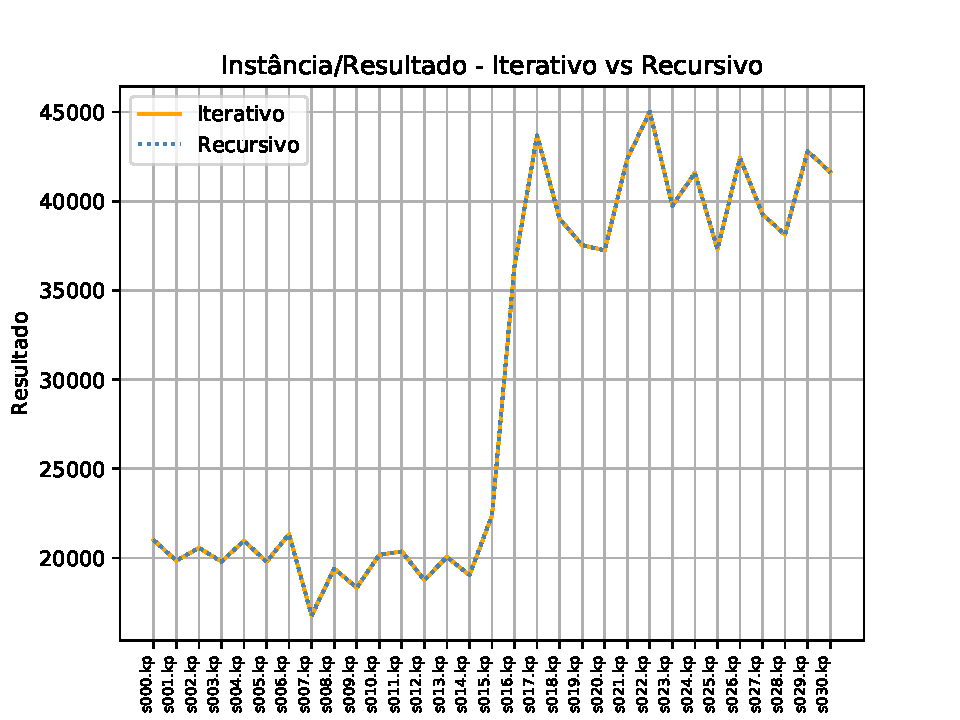
\includegraphics[width=0.6\textwidth]{../img/result_two.pdf}
    \caption{Gráfico do Resultado/Instância}
    \label{fig:result_two}
\end{figure}

Como podemos ver, o tempo necessário para atingir os mesmos resultados são bem maiores quando
comparamos o \nameref{sec:topdown} ao \nameref{sec:bottomup}, computacionalmente falando. Porém, era de
se esperar um resultado como esse, como vimos na página \pageref{sec:introducao} as características de cada um.

\begin{figure}[!htb]
    \centering
    \begin{minipage}{0.55\textwidth}
        \centering
        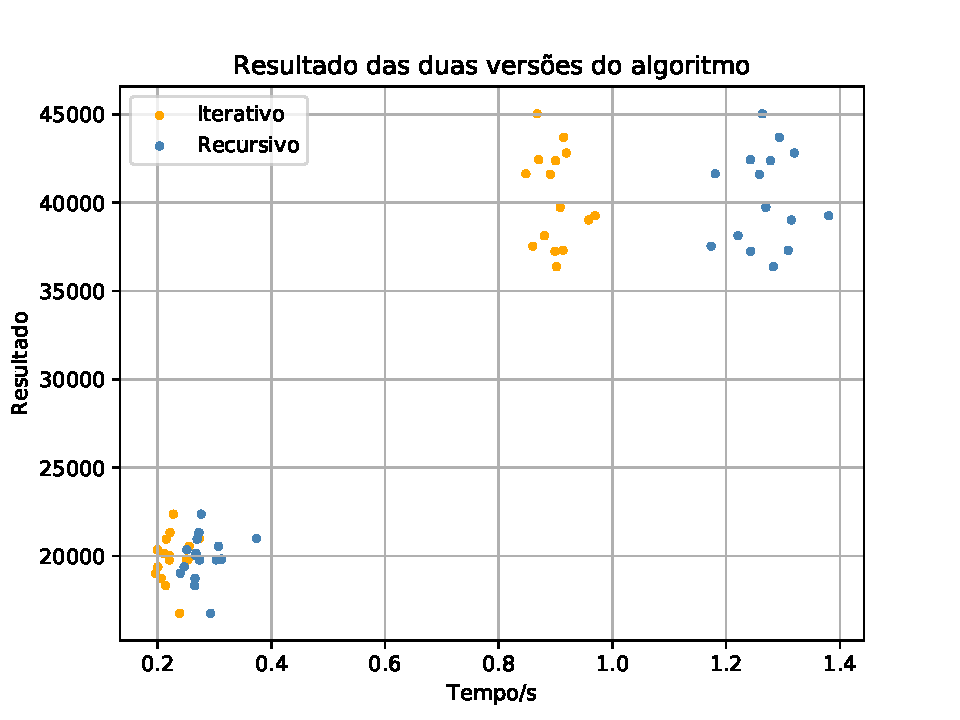
\includegraphics[width=1\textwidth]{../img/scatter_two.pdf}
        \caption{\footnotesize{Gráfico do Tempo/Resultado}}
        \label{fig:scatter_two} 
    \end{minipage}%
    \begin{minipage}{0.6\textwidth}
        \centering
        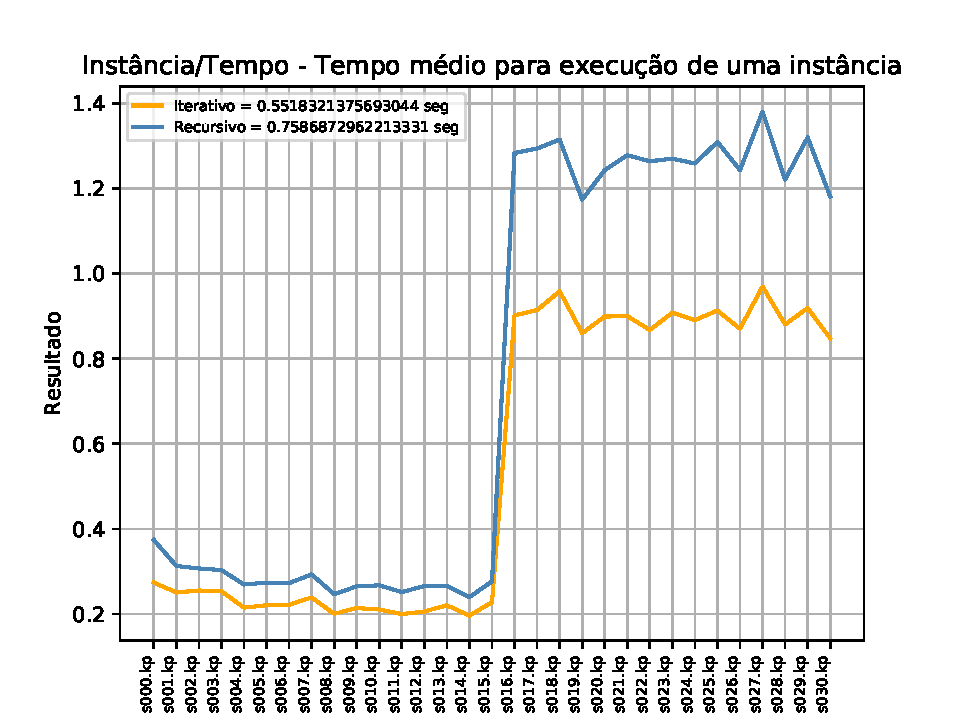
\includegraphics[width=1\textwidth]{../img/time_two.pdf}
        \caption{\footnotesize{Gráfico do Tempo/Instância}}
        \label{fig:time_two}
    \end{minipage}
\end{figure}
\newpage
\subsection{Exprimindo Resultados}
A fim de comprovar o comportamento dos gráficos, decidi executar {\bf 100 vezes} as instâncias com o objetivo de minimizar
a variação do tempo de execução de cada instância.

Para cada instância é armazenado seu tempo de execução individual, logo, foi necessário a cada execução somar o tempo
de cada instância para obter o tempo gasto para esse algoritmo para uma única execução. Feito isso, bastou
repetir o mesmo processo para todas iterações. Assim, obtive o tempo total de execução para os dois algoritmos. O tempo
médio é em relação ao tempo que uma única instância gastou em 100 execuções.
%%%%%%%%%%%%%%%%%%%%%%%%%%%%%%%%%%%%%%%%%%%%%%%%%%%%%%%%%%%%%%%%%%%%%%%%%%%%%%%%%%%%%%%%%%%%%%%%%%%%%%
\subsection{Top-Down}
\begin{table}[!htb]
    \begin{tabular}{ll}
        {\bf Tempo total de execução}: 39 minutos\\
        {\bf Tempo médio gasto por cada instância no total}: 1 minuto e 25 seg
    \end{tabular}
    \caption{Tempo total}
    \label{tab:total_topdown}
\end{table}

Após coletar os dados de todas as execuções, foi se calculado a média total para cada item e obtido um resultado 
mais exprimido a fim de minimizar a variação.
\begin{table}[!htb]
    \begin{tabular}{ll}
        {\bf Tempo de execução minimizado}: 23.4056 segundos\\
        {\bf Média de execução por instância}: 0.7550 segundos\\
        {\bf Maior tempo gasto por uma das instâncias}: 1.3737 segundos\\
        {\bf Menor tempo gasto por uma das instâncias}: 0.2419 segundos \\
        {\bf Instância com maior tempo de execução}: s027.kp\\
        {\bf Instância com menor tempo de execução}: s014.kp
    \end{tabular}
    \caption{Resultados a partir de 100 execuções}
    \label{tab:result_tot_topdown}
\end{table}

\vspace{-15pt}

\begin{table}[!htb]
    \begin{tabular}{ll}
        {\bf Amplitude}: 1.1317 segundos\\
        {\bf Erro}: 0.0905 segundos\\
        {\bf Variância}: 0.2457 segundos\\
        {\bf Desvio Padrão}: 0.4957 segundos\\
        {\bf Desvio Absoluto}: 0.1431 segundos
    \end{tabular}
    \caption{Estatísticas}
    \label{tab:estatistica_tot_topdown}
\end{table}
\newpage
%%%%%%%%%%%%%%%%%%%%%%%%%%%%%%%%%%%%%%%%%%%%%%%%%%%%%%%%%%%%%%%%%%%%%%%%%%%%%%%%%%%%%%%%%%%%%%%%%%%%%%
\subsection{Bottom-Up}
\begin{table}[!htb]
    \begin{tabular}{ll}
        {\bf Tempo total de execução}: 29 minutos\\
        {\bf Tempo médio gasto por cada instância no total}: 55.9276 segundos
    \end{tabular}
    \caption{Tempo total}
    \label{tab:total_bottomup}
\end{table}
% aqui falar do porque de fazer a media...\\
O mesmo processo foi realizado para se obter os dados exprimidos para o {\it Bottom-Up}.
\begin{table}[!htb]
    \begin{tabular}{ll}
        {\bf Tempo de execução minimizado}: 17.3375 segundos\\
        {\bf Média de execução por instância}: 0.5592 segundos\\
        {\bf Maior tempo gasto por uma das instâncias}: 0.9883 segundos\\
        {\bf Menor tempo gasto por uma das instâncias}: 0.1929 segundos \\
        {\bf Instância com maior tempo de execução}: s027.kp\\
        {\bf Instância com menor tempo de execução}: s014.kp
    \end{tabular}
    \caption{Resultados a partir de 100 execuções}
    \label{tab:result_tot_bottomup}
\end{table}

\vspace{-15pt}

\begin{table}[!htb]
    \begin{tabular}{ll}
        {\bf Amplitude}: 0.7953 segundos\\
        {\bf Erro}: 0.0635 segundos\\
        {\bf Variância}: 0.1209 segundos\\
        {\bf Desvio Padrão}: 0.3478 segundos\\
        {\bf Desvio Absoluto}: 0.1188 segundos
    \end{tabular}
    \caption{Estatísticas}
    \label{tab:estatistica_tot_bottomup}
\end{table}
\newpage
% \clearpage
\section{Resultados Obtidos}
Ao anasilar as tabelas \ref{tab:topdown_exec}, \ref{tab:bottomup_exec} que mostram os resultados a
partir da execução de uma única instância, podemos ver que mesmo após 100 execuções, o comportamento geral
se mantém, como podemos ver nas tabelas \ref{tab:result_tot_topdown} e \ref{tab:result_tot_bottomup}.
Tendo estes resultados \dots

\begin{figure}[!htb]
    \centering
    \includegraphics[width=0.6\textwidth]{../img/avg_scatter.pdf}
    \caption{Gráfico do Resultado/Instância}
    \label{fig:avg_scatter}
\end{figure}
\begin{figure}[!htb]
    \centering
    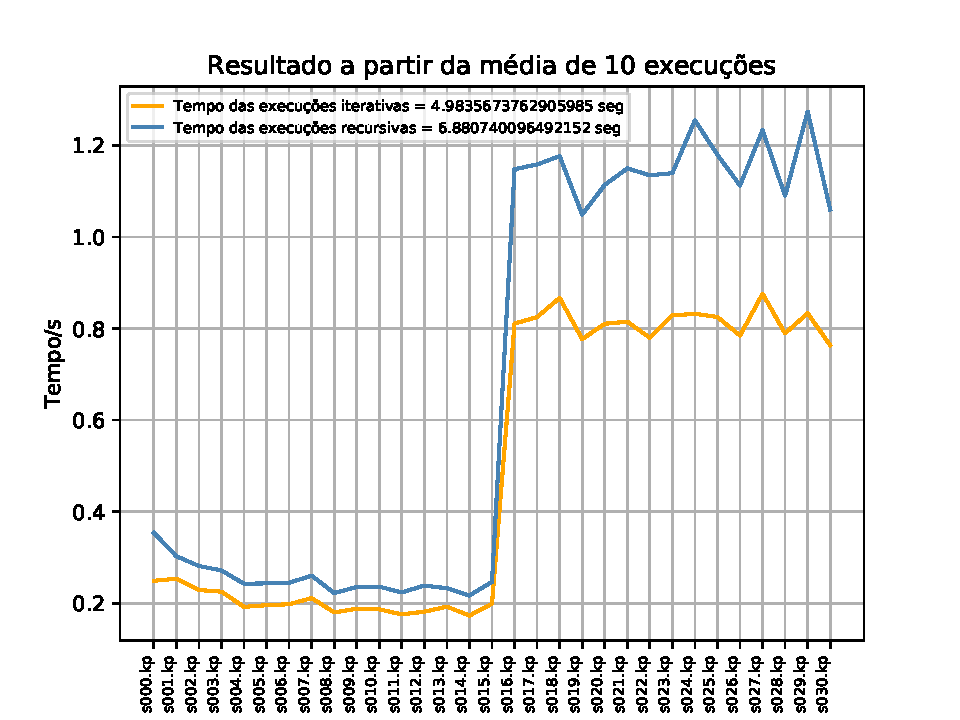
\includegraphics[width=0.8\textwidth]{../img/avg_result.pdf}
    \caption{Gráfico do Resultado/Instância}
    \label{fig:avg_result}
\end{figure}
\clearpage

\subsection{Resultados Finais}


\begin{figure}[!htb]
    \centering
    \includegraphics[width=0.82\textwidth]{../img/mixed_scatter.pdf}
    \caption{Gráfico do Resultado/Instância}
    \label{fig:mixed_scatter}
\end{figure}

falar dos dados estatisticos e comparar o tempo do max e min, antes de fazer a media ..........
\begin{figure}[!htb]
    \centering
    \includegraphics[width=0.82\textwidth]{../img/mixed_result.pdf}
    \caption{Gráfico do Resultado/Instância}
    \label{fig:mixed_result}
\end{figure}

\end{document}